\documentclass[9pt]{beamer}
\usetheme{Madrid}
\usefonttheme{serif}

\usepackage{fontspec}
% надёжный шрифт с кириллицей (работает в Overleaf)
\setmainfont{Libertinus Serif}[Ligatures=TeX]
\setsansfont{Libertinus Sans}[Ligatures=TeX]
\newfontfamily\cyrillicfont{Libertinus Serif}
\newfontfamily\cyrillicfontsf{Libertinus Sans}
\usepackage{polyglossia}
\setmainlanguage{russian}
\setotherlanguage{english}

\usepackage{amsmath}
\usepackage{amsfonts}
\usepackage{amssymb}
\usepackage{graphicx}
\usepackage{microtype}

\usepackage{xcolor}
\usepackage{pifont}
\usepackage{tikz}
\newcommand{\plus}{\tikz[baseline=(X.base)] \node[fill=green!65!black, rounded corners=2pt, inner sep=2pt] (X) {\color{white}\ding{51}};}
\newcommand{\minus}{\tikz[baseline=(X.base)] \node[fill=red!70!black,   rounded corners=2pt, inner sep=2pt] (X) {\color{white}\ding{55}};}

\DeclareMathOperator{\sen}{sen}
% \DeclareMathOperator{\tg}{tg}

\setbeamertemplate{caption}[numbered]

% --- Информация о презентации ---
\author[Автор]{Чиняев Владимир Николаевич}
\title{Линейное приближение. Одноимпульсные манёвры}
\newcommand{\coursename}{Введение в маневрирование} % <-- Поставь здесь нужное название курса
\setbeamertemplate{navigation symbols}{} 
\institute[]{Московский физико технический институт} 
\date{16 сентября 2025 г.} 

\bibliographystyle{apalike}

% --- Кастомная нижняя синяя полоска: курс слева, номер слайда справа ---
\setbeamertemplate{footline}{
  \leavevmode%
  \begin{beamercolorbox}[wd=\paperwidth,ht=2ex,dp=1ex]{palette primary}
    \hspace{0.4cm}\usebeamerfont{footline}\coursename\hfill\usebeamerfont{footline}\insertframenumber\hspace{0.4cm}
  \end{beamercolorbox}%
}

% Чтобы убрать лишние отступы в footer-шрифте (опционально)
\setbeamerfont{footline}{size=\small}

\begin{document}

\begin{frame}
\titlepage
\end{frame}

\begin{frame}{Общая постановка задачи перехода}
Рассмотрим обыкновенное дифференциальное уравнение, краевые условия, ограничения:
\begin{gather*}
    \dot{\mathbf{y}} = \mathbf{f}(t, \mathbf{y}) + \mathbf{u}(t), \\
    \mathbf{y}(t_i) = \mathbf{y}_i = \left( \textbf{Э}_i, \nu_i \right)^T, \\
    \textbf{Э}_t - \text{целевая орбита}, \\
    \mathbf{y}(t) \preceq \mathbf{h}(t),
\end{gather*}
где $\mathbf{y}(t) = \left( \textbf{Э}(t), \nu(t) \right)^T$ \textemdash\ вектор состояния, $\textbf{Э}(t)=\left( a(t), e(t), i(t), \omega(t), \Omega(t) \right)^T$ \textemdash\ параметры кеплеровой орбиты, $\mathbf{f}(t, \mathbf{y})$ \textemdash\ правая часть пассивного движения, $\mathbf{u}(t)$ \textemdash\ управляющая функция, $\mathbf{h}(t)$ \textemdash\ вектор ограничений на состояние КА. Необходимо найти такую управляющую функцию $\mathbf{u}^*(t)$, что функционал 
\begin{equation*}
    \int_{t_i}^{t_f} |\Delta V(\mathbf{u}^*(t))| dt \to \min,
\end{equation*}
будет достигать минимального значения при выполнении условия $\textbf{Э}(t_f)=\textbf{Э}_t$, где $\Delta V = \Delta V(\mathbf{u}(t))$ \textemdash\ функция характеристической скорости.
\end{frame}

\begin{frame}{Цилиндрическая система координат}
\begin{columns}[T,onlytextwidth]
  % левая колонка
  \begin{column}{0.50\textwidth}
    \begin{center}
        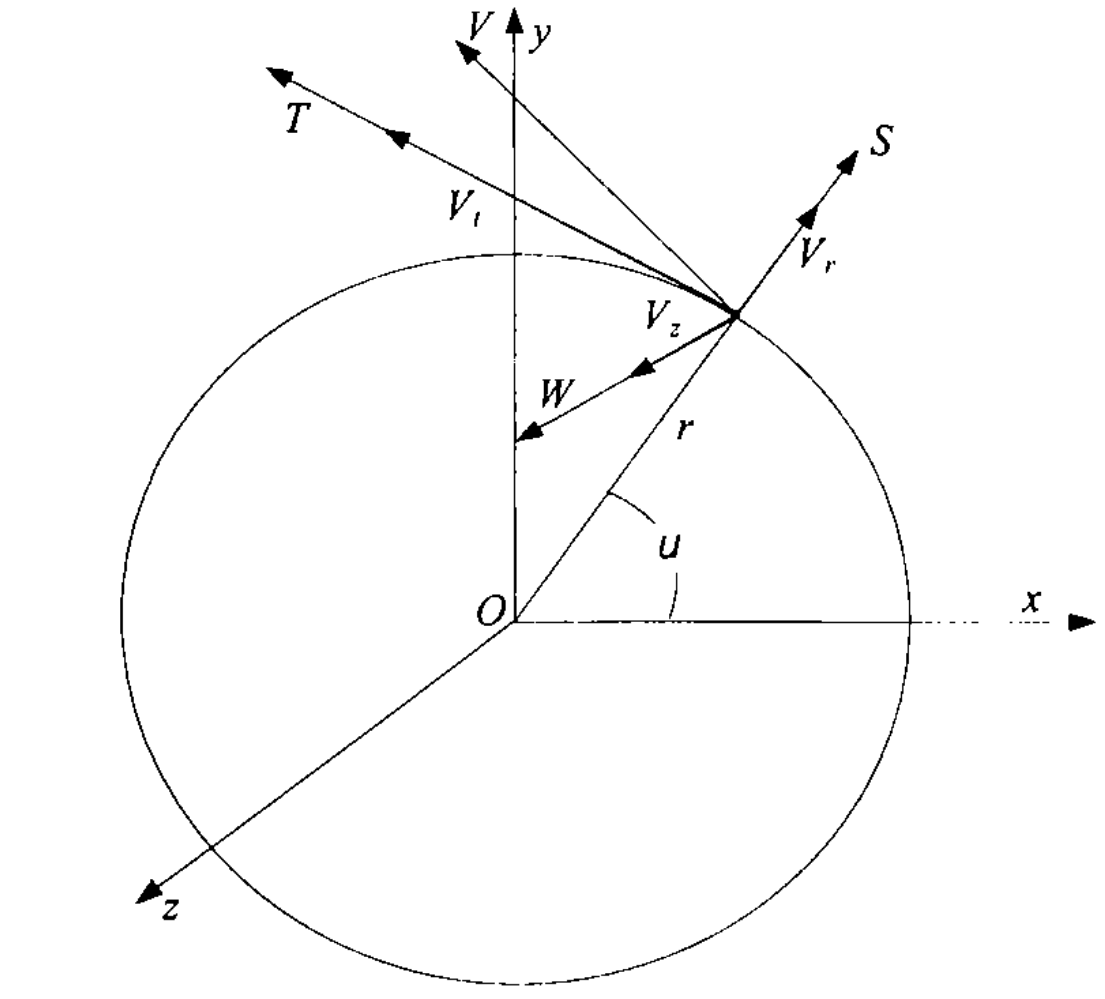
\includegraphics[height=0.60\textheight,keepaspectratio]{images/2/cyl_sk.png}
    \end{center}
  \textbf{Невозмущённая орбита} \textemdash\ круговая орбита радиуса $r$.
  \end{column}

  % правая колонка
  \begin{column}{0.50\textwidth}
  Обозначения:
  \begin{itemize}
      \item $r$ \textemdash\ расстояние от центра Земли до проекции спутника на плоскость невозмущённой орбиты;
      \item $u$ \textemdash\ угол, отсчитываемый в плоскости невозмущённой орбиты от некоторой начальной оси Ox по направлению полёта спутника;
      \item $z$ \textemdash\ расстояние от плоскости невозмущённой орбиты до спутника;
      \item $S$, $T$, $W$ \textemdash\ проекции возмущающих ускорений на оси орбитальной СК.
  \end{itemize}  
  \textbf{Возмущающим ускорением} будем считать суммарное ускорение, возникающее в  результате действия всех сил за исключением силы, создаваемой центральным гравитационным полем $\left( g = \frac{\mu}{r^2} \right)$.
  \end{column}
\end{columns}
\end{frame}

\begin{frame}{Система уравнений движения в кеплеровых элементах}
\begin{equation*}
    \begin{aligned}
        \frac{da}{dt} &= \sqrt{\frac{p}{\mu}} \frac{2a}{1 - e^2} \left( S e \sin \nu + T \frac{p}{r} \right), \\
        \frac{de}{dt} &= \sqrt{\frac{p}{\mu}} \left\{ S \sin \nu + T \left[ \left(1 + \frac{r}{p} \right) \cos \nu + e \frac{r}{p} \right] \right\}, \\
        \frac{d \omega}{dt} &= \sqrt{\frac{p}{\mu}} \left\{ -S \frac{\cos \nu}{e} + T \frac{1}{e}  \left(1 + \frac{r}{p} \right) \sin \nu - W \frac{r}{p} \text{ctg } i \sin u  \right\}, \\
        \frac{d \Omega}{dt} &= W \sqrt{\frac{p}{\mu}} \frac{r}{p} \frac{\sin u}{\sin i}, \\
        \frac{d i}{dt} &= W \sqrt{\frac{p}{\mu}} \frac{r}{p} \cos u, \\
        \frac{d \nu}{dt} &= \sqrt{\frac{p}{\mu}} \left\{ \frac{\mu}{r^2} +  S \frac{\cos \nu}{e} - T \frac{1}{e} \left(1 + \frac{r}{p} \right) \sin \nu \right\}, \\
        ||| \frac{d M}{dt} &= n + \sqrt{\frac{p}{\mu}} \frac{\sqrt{1 - e^2}}{e} \left\{ \left( \cos \nu - 2e \frac{r}{p} \right) S - \left(1 + \frac{r}{p} \right) \sin \nu T \right\} |||
    \end{aligned}
\end{equation*}
где 
\begin{equation*}
    r = \frac{p}{1 + e \cos \nu}, \quad p = a (1 - e^2), \quad u = \omega + \nu.
\end{equation*}
\end{frame}

\begin{frame}{Система уравнений в цилиндрической СК}
Считая отношение $\frac{z}{r}$ малым, и пренебрегая величинами второго порядка малости, можно написать уравнения движения КА во введённой системе координат \cite{Suslov}:
\begin{equation*}
    \begin{aligned}
        S - g &= \ddot{r} - r\dot{u}^2, \\
        T &= \frac{1}{r} \frac{d}{dt} (r^2 \dot{u}), \\
        W &= \ddot{z} + g \frac{z}{r}.
    \end{aligned}
\end{equation*}
Введём дополнительные предположения:
\begin{itemize}
    \item Возмущающие ускорения $S, T, W$ малы по сравнению с $g$;
    \item Отклонения от кругового движения, вызываемые $S, T, W$ малы по сравнению с $r_0$;
    \item С точностью до малых первого порядка не учитываем влияние на $S, T, W$ отклонений возмущённой орбиты от невозмущённой круговой орбиты.
\end{itemize}
\end{frame}

\begin{frame}{Система уравнений в цилиндрической СК}
Обозначим через
\begin{equation*}
    V_r = \dot{r} \quad \quad V_t = r \dot{u}
\end{equation*}
проекции вектора скорости соответственно на направление радиус-вектора и нормаль к нему в плоскости невозмущённой орбиты. Подставляя эти величины в первые два уравнения предыдущей системы и используя описанные выше предположения, получим:
\begin{gather*}
    \dot{V}_r = S - \frac{\mu}{r^2} + \frac{V_t^2}{r}, \\
    \dot{V}_t = T - \frac{V_t V_r}{r}, \\
    \dot{r} = V_r, \\
    \dot{u} = \frac{V_t}{r}.
\end{gather*}
Эта система четёрых дифференциальных уравнений относительно неизвестных $r, V_r, V_t, u$ \textbf{не решается в конечном виде} при произвольных значениях возмущающих ускорений $S$ и $T$.
\end{frame}

\begin{frame}{Уравнения движения в отклонениях от движения по круговой орбите}
Для построения приближённого решения системы уравнений, полученной выше, предположим, что основные характеристики рассматриваемого возмущённого движения на интересующем интервале времени мало отличаются от соответствующих характеристик движения по невозмущённой круговой орбите. Обозначим через $\Delta r, \Delta V_r, \Delta V_t, \Delta u$ разности между значениями соответствующих величин для возмущённой и невозмущённой орбит:
\begin{equation*}
    r = r_0 + \Delta r, \quad \quad V_r = \Delta V_r, \quad \quad V_t = V_0 + \Delta V_t.
\end{equation*}
Тогда мы можем получить:
\begin{gather*}
    \Delta \dot{V}_r - 2 \lambda_0 \Delta V_t - \lambda_0^2 \Delta r = S, \\
    \Delta \dot{V}_t + \lambda_0 \Delta V_r = T, \\
    \Delta \dot{r} - \Delta V_r = 0, \\
    \Delta \dot{u} = \frac{1}{r_0} \left( \Delta V_t - \lambda_0 \Delta r \right), \\
    \ddot{z} + \lambda_0^2 z = W, \\
    V_z = \dot{z},
\end{gather*}
где $\lambda_0 = \frac{V_0}{r_0}$ \textemdash\ угловая скорость движения КА по круговой невозмущённой орбите. \\
Мы получили систему линейных дифференциальных уравнений с постоянными коэффициентами относительно неизвестных $\Delta r, \Delta V_r, \Delta V_t, \Delta u, \Delta z, \Delta V_z$.
\end{frame}

\begin{frame}{Решение системы дифференциальных уравнений}
\begin{columns}[T,onlytextwidth]
  % левая колонка
  \begin{column}{0.50\textwidth}
    \begin{gather*}
        \sum_{j=1}^{N} \Bigl( \Delta V_{rj} \sin \phi_j + 2 \Delta V_{tj} \cos \phi_j \Bigl) = V_0 \Delta e_x, \\
        \sum_{j=1}^{N} \Bigl( -\Delta V_{rj} \cos \phi_j + 2 \Delta V_{tj} \sin \phi_j \Bigl) = V_0 \Delta e_y, \\
        \sum_{j=1}^{N} 2 \Delta V_{tj} = V_0 \Delta a, \\
        \sum_{j=1}^{N} (2 \Delta V_{rj} (1 - \cos \phi_j) + \Delta V_{tj} (-3 \phi_j + 4 \sin \phi_j)) = \Delta t, \\
        \sum_{j=1}^{N} -\Delta V_{zj} \sin \phi_j = 0, \\
        \sum_{j=1}^{N} \Delta V_{zj} \cos \phi_j = V_0 \Delta i.
    \end{gather*}
  \end{column}

  % правая колонка
  \begin{column}{0.45\textwidth}
    Обсуждение:
    \begin{itemize}
        \item Система была получена "слева - направо": исследовали конечные приращения вектора скорости $\longrightarrow$ получили конечные приращения элементов орбиты;
        \item В маневрировании с этой системой работают "справа - налево": имеем необходимые изменения орбитальных элементов $\longrightarrow$ находим импульсы скорости и углы их приложения;
        \item Система имеет $4N$ неизвестных \textemdash\ $N * (\Delta V_{rj}, \Delta V_{tj}, \Delta V_{zj}, \phi_j)$;
        \item Тип системы \textemdash\ СНАУ, если положить углы $\phi_j$ известными, система станет СЛАУ.
    \end{itemize}
  \end{column}
\end{columns}

\end{frame}

\begin{frame}{Отклонения орбитальных элементов}
Введём опорную орбиту \textemdash\ круговую орбиту с радиусом $r_0 = (a_i + a_t) / 2$. Скорость движения тела по такой орбите определяется выражением $V_0 = \sqrt{\mu / r_0}$, где $\mu$ \textemdash\ гравитационный параметр центрального тела. Отклонение большой полуоси $\Delta a$ зададим следующим выражением:
\begin{equation*}
    \Delta a = \frac{a_t - a_i}{r_0}.
\end{equation*}
Отклонение вектора эксцентриситета:
\begin{equation*}
    \Delta e = \sqrt{\Delta e_x^2 + \Delta e_y^2}.
\end{equation*}
Его проекции задаются выражениями
\begin{gather*}
    \Delta e_x = e_t \cos \omega_t - e_i \cos \omega_i, \\
    \Delta e_y = e_t \sin \omega_t - e_i \sin \omega_i.
\end{gather*}
\end{frame}

\begin{frame}{Отклонения орбитальных элементов}

\begin{center}
    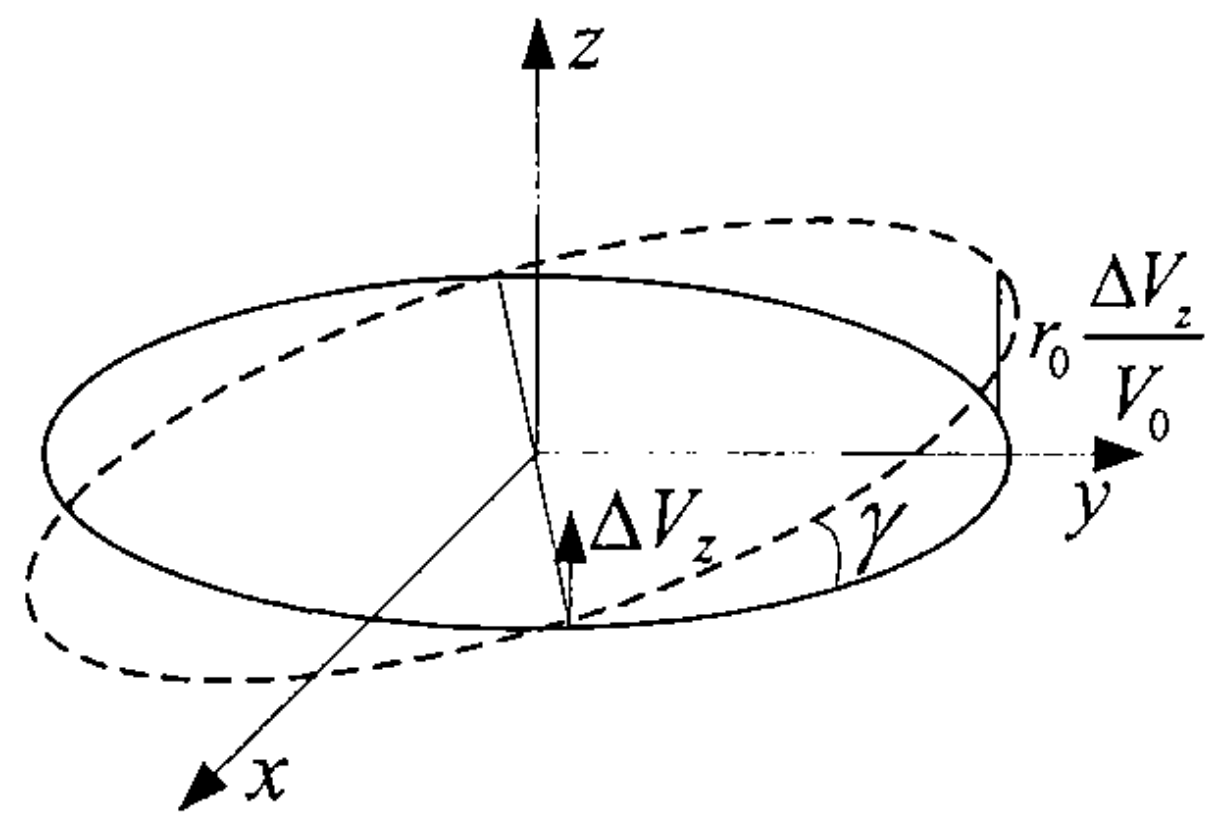
\includegraphics[height=0.40\textheight,keepaspectratio]{images/2/orb_dVn.png}
\end{center}

Используя сферическую формулу косинусов, найдём угол $\Delta \gamma$ между плоскостями двух орбит:
    \begin{equation*}
        \cos \Delta \gamma = \cos i_t \cos i_i + \sin i_t \sin i_i \cos (\Omega_t - \Omega_i).
    \end{equation*}
    И определим изменение наклонения в согласии с \cite{Baranov}:
    \begin{equation*}
        \Delta i = 2 \sin \frac{\Delta \gamma}{2}.
    \end{equation*}
    Важно заметить, что величина $\Delta i$ учитывает как наклонения, так и долготы восходящих узлов начальной и целевой орбит. Определение $\Delta i$ удобно и часто используется, так как для малых $\Delta \gamma$ величина $\Delta i \approx \Delta \gamma$, а для всех углов от $0$ до $2 \pi$  это непрерывная гладкая функция абсолютного значения $\Delta \gamma$.
\end{frame}

\begin{frame}{Задачи перехода в линейной постановке}
Рассмотрим обыкновенное дифференциальное уравнение и краевые условия:
\begin{gather*}
    \dot{\mathbf{y}} = \mathbf{f}(t, \mathbf{y}) + \mathbf{u}(t), \\
    \mathbf{y}(t_i) = \mathbf{y}_i = \left( \textbf{Э}_i, \nu_i \right)^T, \quad \quad
    \textbf{Э}_t - \text{целевая орбита},
\end{gather*}
где $\mathbf{y}(t) = \left( \textbf{Э}(t), \nu(t) \right)^T$ \textemdash\ вектор состояния, $\textbf{Э}(t)=\left( a(t), e(t), i(t), \omega(t), \Omega(t) \right)^T$ \textemdash\ параметры кеплеровой орбиты, $\mathbf{f}(t, \mathbf{y}) = (0 \; ... \; 0 \; \dot{\nu} )$ \textemdash\ правая часть пассивного движения, $\mathbf{u}(t) = \sum_{j=1}^N \delta(t - t_j) \mathbf{g}_j$ \textemdash\ управляющая функция, $\mathbf{g}_j$ \textemdash\ скорость изменения орбитальных элементов в ходе приложения $j$-го точечного импульса. Необходимо найти такую управляющую функцию $\mathbf{u}^*(t)$, что суммарная характеристическая скорость 
\begin{equation*}
    \Delta V (\mathbf{u}^*(t)) = \sum_{j=1}^N \sqrt{\Delta V_{rj}^2 + \Delta V_{tj}^2 + \Delta V_{zj}^2} \to \min,
\end{equation*}
будет достигать минимального значения при выполнении условий:
\begin{gather*}
        \sum_{j=1}^{N} \Bigl( \Delta V_{rj} \sin \phi_j + 2 \Delta V_{tj} \cos \phi_j \Bigl) = V_0 \Delta e_x, \quad \quad
        \sum_{j=1}^{N} \Bigl( -\Delta V_{rj} \cos \phi_j + 2 \Delta V_{tj} \sin \phi_j \Bigl) = V_0 \Delta e_y, \\
        \sum_{j=1}^{N} 2 \Delta V_{tj} = V_0 \Delta a, \quad \quad
        \sum_{j=1}^{N} -\Delta V_{zj} \sin \phi_j = 0, \quad \quad
        \sum_{j=1}^{N} \Delta V_{zj} \cos \phi_j = V_0 \Delta i.
    \end{gather*}
\end{frame}

\begin{frame}{Оптимальное импульсное маневрирование}
Задача нахождения (оптимального) импульсного маневрирования, в соответствии с \cite{Edelbaum_1}, предполагает ответ на 4 вопроса:
\begin{enumerate}
    \item Какое количество импульсов должно быть приложено?
    \item Где они должны быть приложены?
    \item Куда они должны быть направлены?
    \item Как суммарный импульс должен быть распределён, если осуществляется более одного манёвра?
\end{enumerate}
\end{frame}

\begin{frame}{Сколько импульсов?}
Первый из этих вопросов является самым сложным. Он был рассмотрен Эдельбаумом в работе "How many impulses?" \cite{How_many_impulses}. \\
В общем случае неизвестно, как много манёвров требуется для осуществления импульсного перехода (встречи), но в случае линейной задачи известно \cite{Neustadt} \cite{Stern}, что оптимальное маневрирование можно осуществить за число импульсов, равное числу переменных состояния задачи:
\begin{itemize}
    \item Компланарный переход: 3 \textemdash\ $a, e, \omega$;
    \item Некомпланарный переход: 5 \textemdash\ $a, e, \omega, i, \Omega$;
    \item Компланарная встреча: 4 \textemdash\ $a, e, \omega, \nu$;
    \item Некомпланарная встреча: 6 \textemdash\ $a, e, \omega, i, \Omega, \nu$;
\end{itemize}
\end{frame}

\begin{frame}{Сколько импульсов?}
\begin{itemize}
    \item \textbf{1 импульс} \\
        \minus\ Позволит осуществить переход лишь между орбитами, имеющими общую точку. \\
        \minus\ Большинство численных экспериментов \cite{Edelbaum_1} показывают, что одноимульсный переход является менее экономичным по сравнению с мультиимпульсными переходами. \\
        \plus\ Лучший вариант с точки зрения надежности выполнения манёвров.
    \item \textbf{$N$ импульсов} \\
        \plus\ Позволят осуществить переход между произвольными эллиптическими орбитами. \\
        \minus\ Может вызывать проблемы с надёжностью и продолжительностью жизненного цикла КА, вследствие многоразового включения ДУ.
\end{itemize}
\end{frame}

\begin{frame}{Изменение большой полуоси}
\begin{itemize}
    \item Изменение большой полуоси происходит \textbf{только} за счёт трансверсальной составляющей импульса скорости;
    \item Величина изменения большой полуоси \textbf{не зависит} от момента приложения импульса;
    \item Радиальная составляющая \textbf{не изменяет} большую полуось;
    \item Величина трансверсальной составляющей находится из уравнения
    \begin{equation*}
        2 \Delta V_t = \Delta a,
    \end{equation*}
    \begin{equation*}
        \Delta V_t = \frac{1}{2} \Delta a.
    \end{equation*}
\end{itemize}
\end{frame}

\begin{frame}{Изменение эксцентриситета}
\begin{itemize}
    \item Изменение эксцентриситета происходит за счёт трансверсальной и радиальной составляющих импульса;
    \item Величина изменения \textbf{существенно зависит} от момента приложения импульса скорости: наиболее эффективно изменять эксцентриситет, прилагая трансверсальную составляющую импульса в перицентре или апоцентре орбиты;
    \item Величина трансверсальной составляющей:
    \begin{equation*}
        \Delta V_t = \pm \frac{1}{2} \Delta e,
    \end{equation*}
    где $\Delta e = \sqrt{\Delta e_x^2 + \Delta e_y^2}$, знак "+" соответствует перицентру орбиты, "-" - апоцентру.
    \item Эффективность изменения эксцентриситета с помощью радиальной составляющей \textbf{вдвое меньше} , но такой импульс не изменяет величину большой полуоси:
    \begin{equation*}
        \Delta V_r = \pm \Delta e.
    \end{equation*}
\end{itemize}
\end{frame}

\begin{frame}{Поворот плоскости орбиты}
\begin{itemize}
    \item Совместить плоскости орбит можно одним импульсом, прикладываемым на линии пересечения плоскостей начальной и конечной орбит;
    \item Величина импульса:
    \begin{equation*}
        \Delta V_z = \pm \Delta i.
    \end{equation*}
\end{itemize}
\end{frame}

\begin{frame}{Влияние радиальной составляющей импульса скорости}
\begin{columns}[T,onlytextwidth]
  % левая колонка
  \begin{column}{0.50\textwidth}
    \begin{center}
        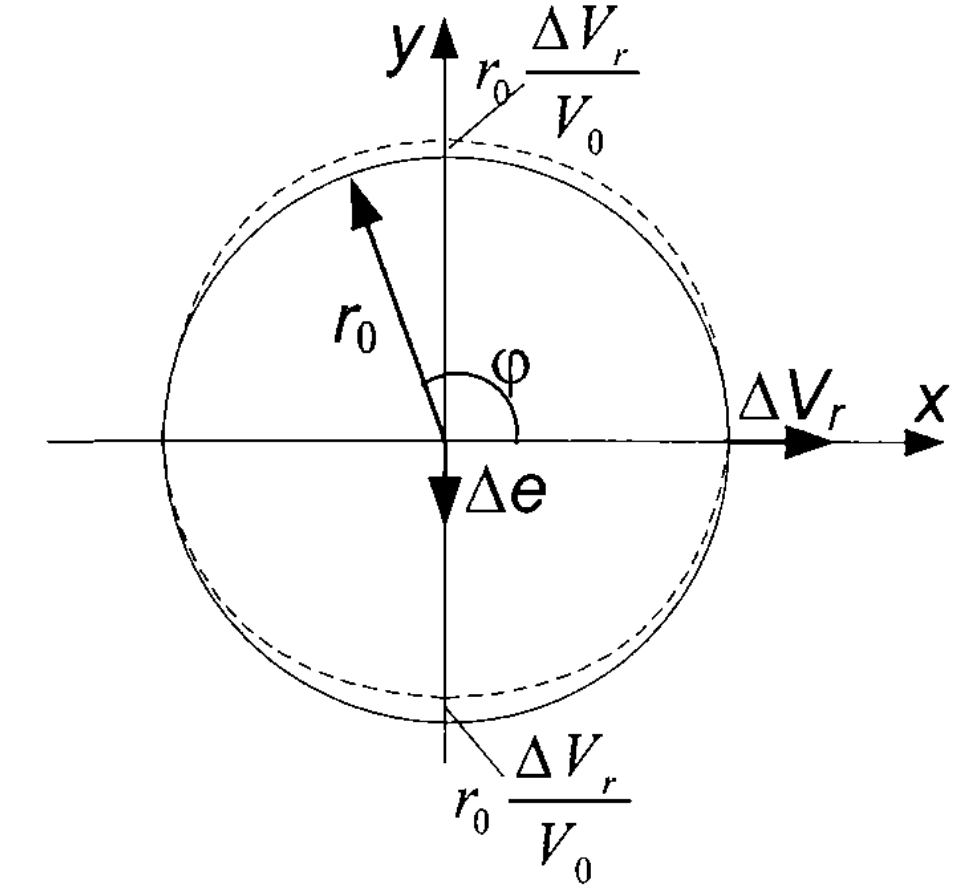
\includegraphics[height=0.50\textheight,keepaspectratio]{images/2/orb_dVr.png}
    \end{center}
    Абсолютные величины отклонений по радиусу в апоцентре и перицентре орбиты равны между собой:
    \begin{equation*}
        \vert \Delta r_{\alpha} \vert = \vert \Delta r_{\pi} \vert = r_0 \frac{\Delta V_r}{V_0}.
    \end{equation*}
  \end{column}

  % правая колонка
  \begin{column}{0.50\textwidth}
    Смещение вдоль орбиты:
    \begin{center}
        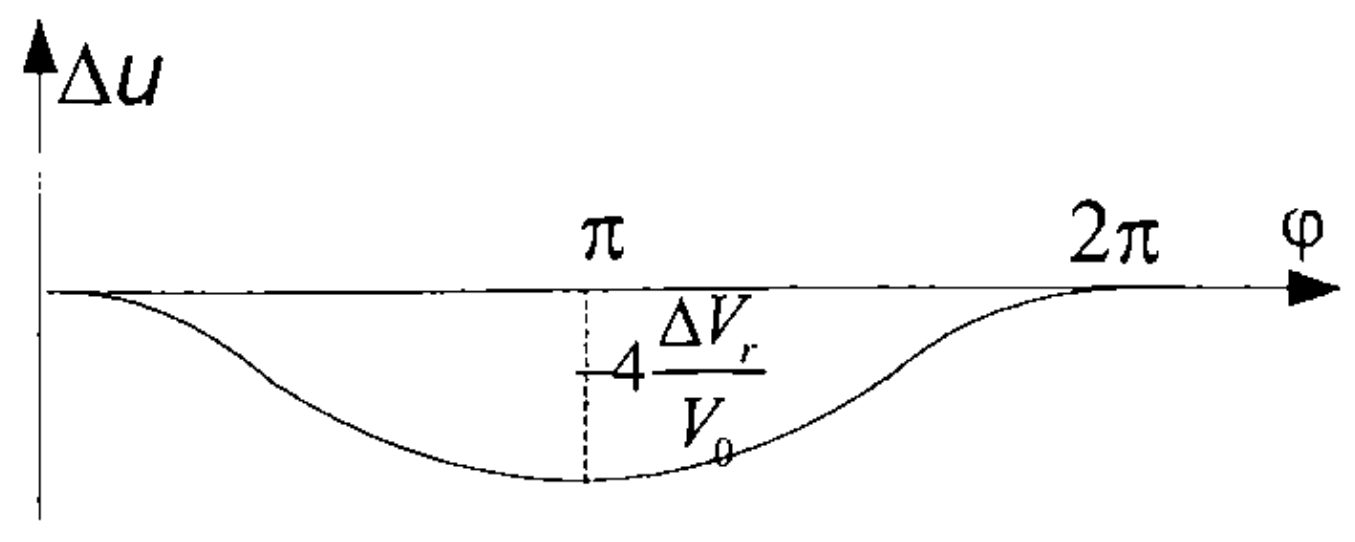
\includegraphics[height=0.25\textheight,keepaspectratio]{images/2/dVr_1.png}
    \end{center}
    После половины витка достигается максимальное отставание от невозмущённого движения:
    \begin{equation*}
        \Delta u = -4 \frac{\Delta V_r}{V_0},
    \end{equation*}
    но к концу витка отставание исчезает, следовательно, \textbf{вековое смещение отсутствует}.
  \end{column}
\end{columns}
\end{frame}

\begin{frame}{Влияние радиальной составляющей импульса скорости}
\begin{columns}[T,onlytextwidth]
  % левая колонка
  \begin{column}{0.50\textwidth}
    Относительное движение:
    \begin{center}
        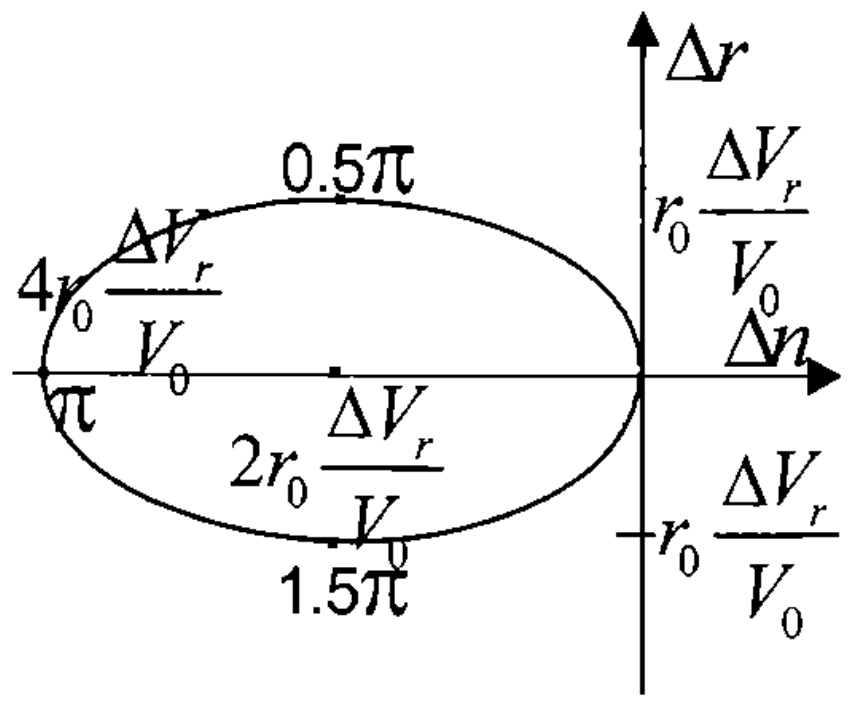
\includegraphics[height=0.35\textheight,keepaspectratio]{images/2/dVr_2.png}
    \end{center}
    \begin{itemize}
        \item $T/4$ \textemdash\ максимальное положительное отклонение по радиусу;
        \item $T/2$ \textemdash\ максимальное отставание вдоль орбиты, нет отклонения по радиусу;
        \item $3T/4$ \textemdash\ максимальное отрицательное отклонение по радиусу;
        \item $T$ \textemdash\ возвращение в исходную точку.
    \end{itemize}
  \end{column}

  % правая колонка
  \begin{column}{0.49\textwidth}
    Пример сближения:
    \begin{center}
        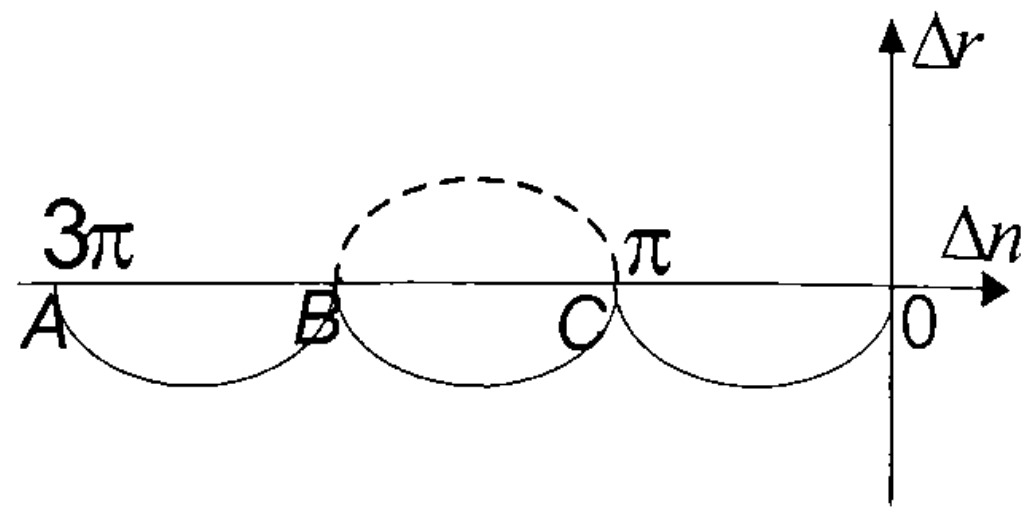
\includegraphics[height=0.30\textheight,keepaspectratio]{images/2/dVr_3.png}
    \end{center}
    \begin{enumerate}
        \item Вывод аппарата на орбиту КА-цели, но позади неё (точка A);
        \item Последовательное приложение отрицательных радиальных импульсов скорости (используются только нижние половины эллипса).
    \end{enumerate}
    Положительная сторона стратегии \textemdash\ \textbf{безопасность КА-цели}.
  \end{column}
\end{columns}
\end{frame}

\begin{frame}{Влияние трансверсальной составляющей импульса скорости}
\begin{columns}[T,onlytextwidth]
  % левая колонка
  \begin{column}{0.50\textwidth}
    \begin{center}
        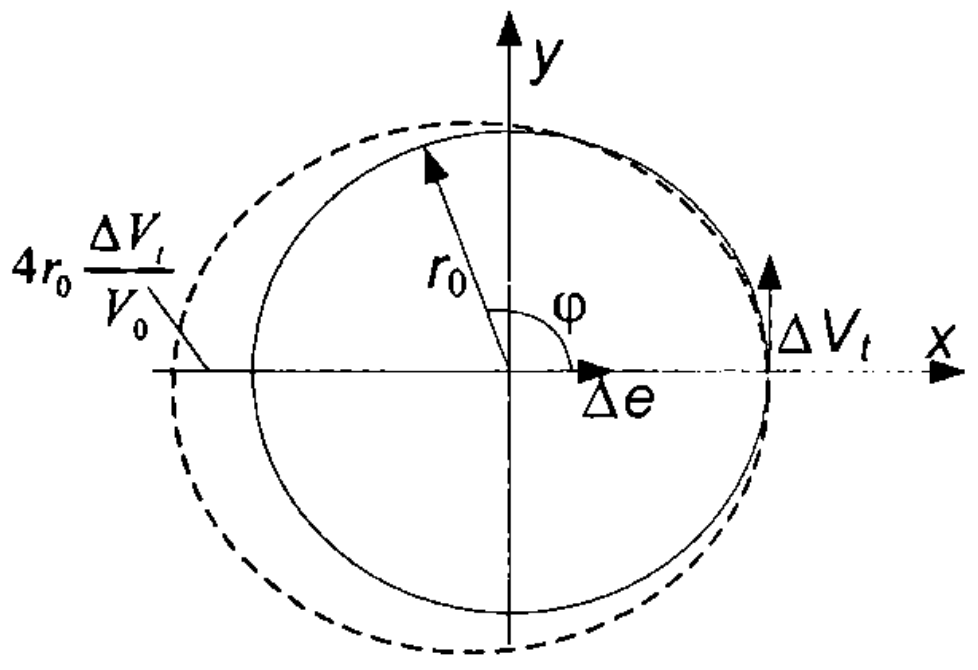
\includegraphics[height=0.40\textheight,keepaspectratio]{images/2/orb_dVt.png}
    \end{center}
    Отклонение по радиусу в апоцентре:
    \begin{equation*}
        \Delta r_{\alpha} = 4 r_0 \frac{\Delta V_t}{V_0}.
    \end{equation*}
  \end{column}

  % правая колонка
  \begin{column}{0.50\textwidth}
    Смещение вдоль орбиты:
    \begin{center}
        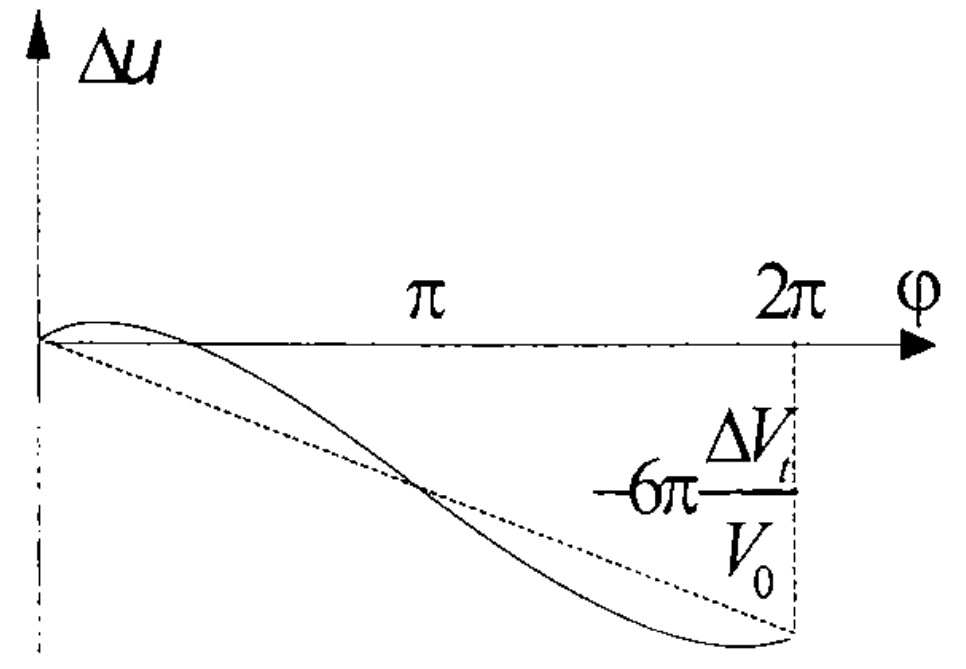
\includegraphics[height=0.35\textheight,keepaspectratio]{images/2/dVt_1.png}
    \end{center}
    Вначале смещение положительно, и достигает своего максимума $\Delta u \approx 0.4776 \frac{\Delta V_t}{V_0}$ при $\phi = 41^{\circ} 24' 35''$, затем смещение вперёд начинает уменьшаться и после $\phi = 73^{\circ} 05' 32''$ начинается отставание от невозмущённого движения. За один виток набирается отставание:
    \begin{equation*}
        \Delta u = -6 \pi \frac{\Delta V_t}{V_0}.
    \end{equation*}
  \end{column}
\end{columns}
\end{frame}

\begin{frame}{Влияние трансверсальной составляющей импульса скорости}
    \begin{center}
        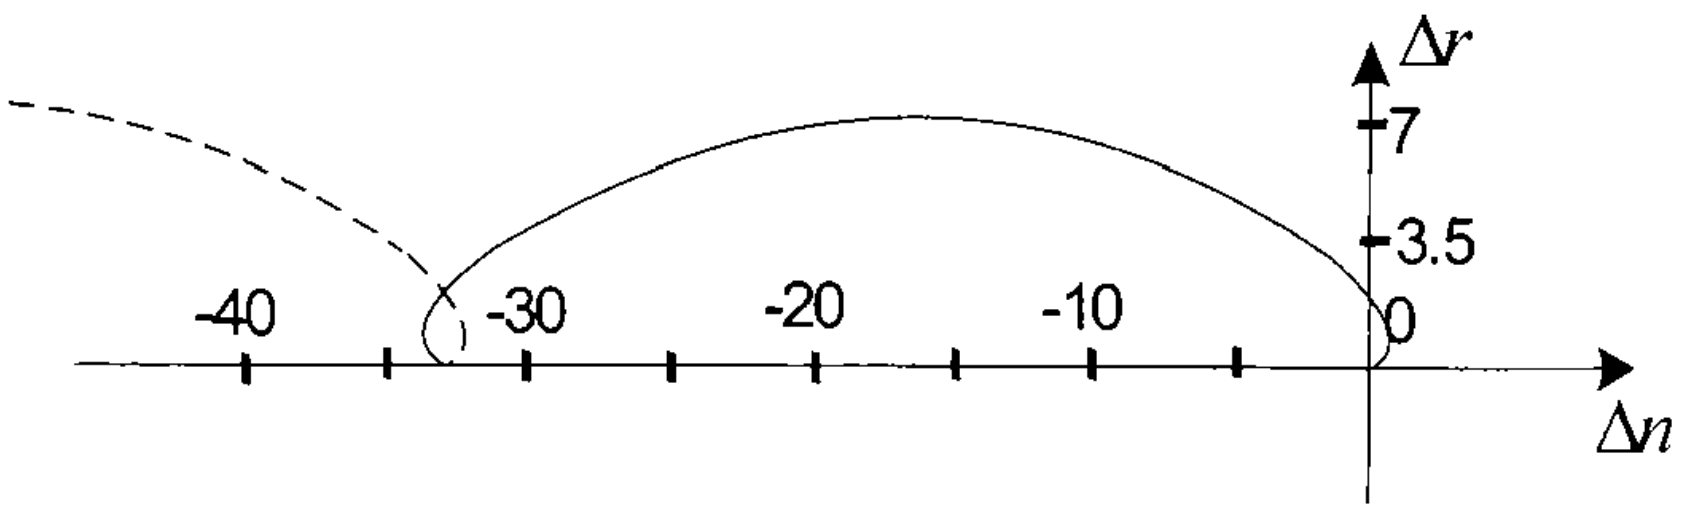
\includegraphics[height=0.30\textheight,keepaspectratio]{images/2/dVt_2.png}
    \end{center}
    На рисунке изображено относительное движение КА, вызванное приложением положительной трансверсальной составляющей импульса ($\Delta V_t = 2 \text{ м/с}$, радиус орбиты $r_0 = 6700$ км). Предмет, брошенный со станции вперёд, сначала будет двигаться вперёд и вверх, затем будет продолжать двигаться вверх, одновременно смещаясь назад, потом будет опускаться и достигнет уровня станции, но позади неё (пунктирная линия - следующий виток).
\end{frame}

\begin{frame}{Влияние боковой составляющей импульса скорости}
    \begin{center}
        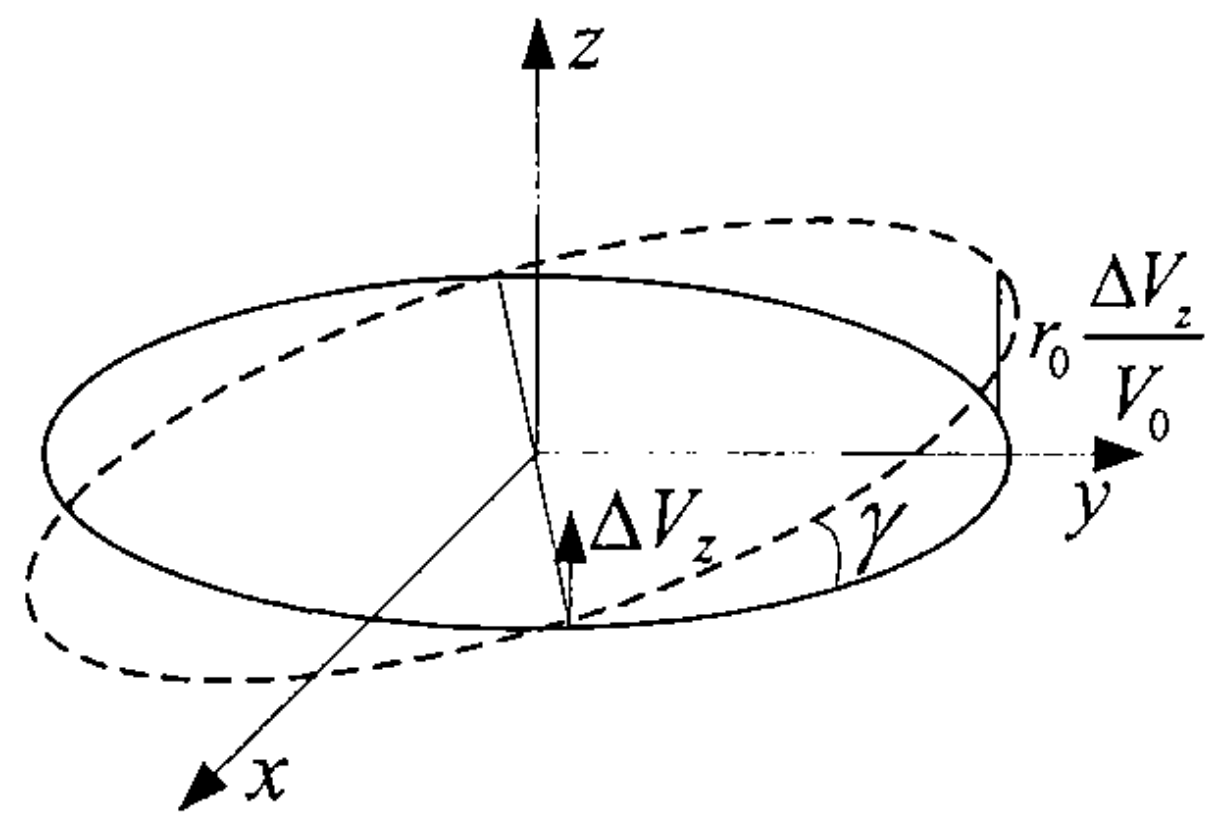
\includegraphics[height=0.30\textheight,keepaspectratio]{images/2/orb_dVn.png}
    \end{center}
    Приложение нормального импульса скорости приводит к повороту плоскости орбиты на угол
    \begin{equation*}
        \gamma \approx \frac{\vert \Delta V_z \vert}{V_0}.
    \end{equation*}
    Максимальное отклонение от плоскости орбиты 
    \begin{equation*}
        \Delta z = r_0 \frac{\vert \Delta V_z \vert}{V_0}.
    \end{equation*}
    Смещения вдоль орбиты не происходит. Относительное движение состоит в колебательном движении вдоль оси $z$, перпендикулярной плоскости орбиты.
\end{frame}

\begin{frame}[allowframebreaks]{Источники}
  \begin{thebibliography}{9}
    \bibitem{How_many_impulses}
    Edelbaum T. How many impulses/ques //3rd and 4th Aerospace Sciences Meeting. – 1967. – С. 7.
    
    \bibitem{Edelbaum_1}
    Edelbaum T. N., Gobetz F. W., Washington M. Minimum-impulse time-free transfer between elliptic orbits. – 1966. – №. NASA-CR-636.

    \bibitem{Neustadt}
    Neustadt L. W. Optimization, a moment problem, and nonlinear programming //Journal of the Society for Industrial and Applied Mathematics, Series A: Control. – 1964. – Т. 2. – №. 1. – С. 33-53.
    
    \bibitem{Stern}
    Stern R. G., Potter J. E. Optimization of midcourse velocity corrections //IFAC Proceedings Volumes. – 1965. – Т. 2. – №. 1. – С. 70-83.

    \bibitem{Suslov}
    Суслов Г. К. Теоретическая механика. – 1946.

    \bibitem{Baranov}
    Баранов А. А. Маневрирование космических аппаратов в окрестности круговой орбиты //М.: Спутник. – 2016.
    
  \end{thebibliography}
\end{frame}

\end{document}
